\begingroup
% Prevent new pages between chapters (in group)
\let\clearpage\relax
\chapter{Introduction}

Three attributes of a secure system (\textblue{CIA}) :
\begin{itemize}
    \item \textblue{Confidentiality} : Cant read/steal data
    \item \textblue{Integrity} : Cant modify data
    \item \textblue{Availability} : Cant disturb access to data
\end{itemize}

\chapter{Access Control}

Access control is about the Confidentiality and Integrity. The goal is to restrict the access to a resource to authorized users only.
This resource can be data or CPU (analogy : steal server resources for mining).
\begin{itemize}
    \item \textblue{Principle of least privileges} : Define the access control rules such that users only have those access rights that they need to do their job (e.g. User "Peter" can access /home/peter but not /home/mary)
    \item \textblue{Implementing access control} : Identify verification via login, Unix file permissions, Access Control Lists (ACL), ...
    \item \textblue{Breaking access control} : Physical (steal computer), Social engineering (convince a legitimate user to five the resource/access right to you), ...
\end{itemize}

\chapter{How a CPU executes programs}

Each running process gets its own virtual address space. When the program is loaded, the OS reserves blocks in main memory. It contains :
\begin{itemize}
    \item \textblue{TEXT} segment (Code of the program)
    \item \textblue{DATA} segment (Constants, ...)
    \item \textblue{HEAP} segment (Dynamically loaded libraries (\ctext{lightGray}{.dll/.so})) : Grows by allocation \textit{manually} memory space (e.g. with \ctext{lightGray}{malloc})
    \item \textblue{STACK} segment (Variables values, ...) : Grow downwards by allocating \textit{automatically} (via 
\end{itemize}

A CPU has several \textblue{registers} (temporary data stores that are used to perform calculations). For the CPU, variables are just locations in main memory. There is a special register that contains the address of the next instruction to be executed, called the \textblue{Instruction Pointer (ip)} (or Program Counter (pc)). Another register, the \textblue{Stack Pointer (sp)} contains the top of the stack's address.

When a function is called, a stack fram is put on the stack during runtime. When $f(3, 4)$ returns, the top stack frame is removed from the stack, and the program execution continues at the instruction stored at the return address. Many CPUs have a \textblue{frame pointer register (fp)} that points at the end of the block with local variables, that allows to easily calculate the address of its local variables and parameters.

\begin{figure}[H]
    \centering
    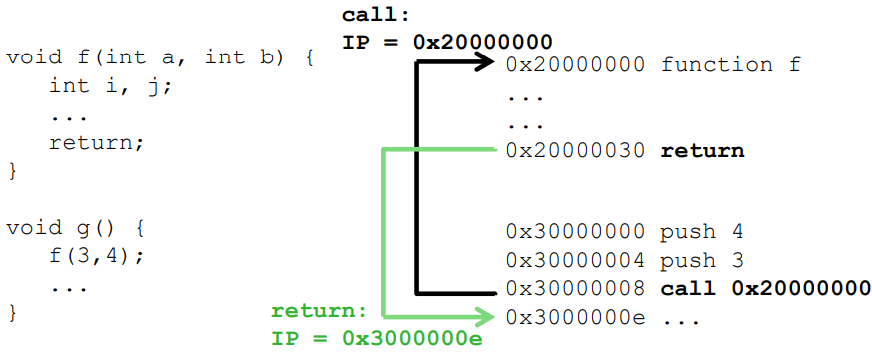
\includegraphics[width=0.55\textwidth,keepaspectratio]{function_call}\hfill
	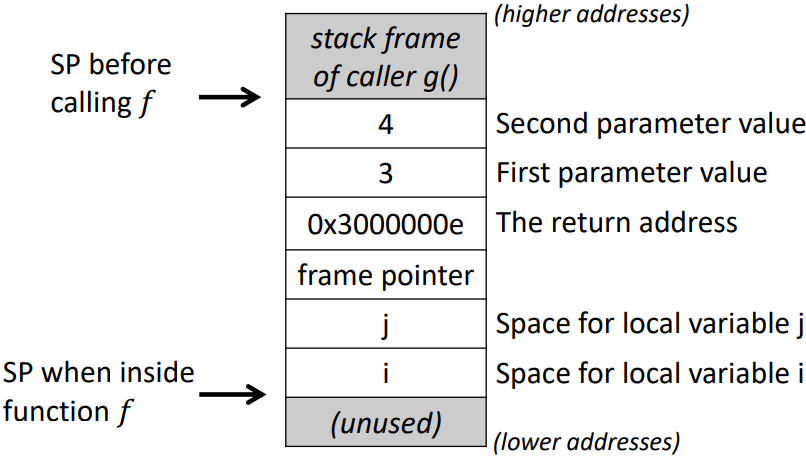
\includegraphics[width=0.45\textwidth,keepaspectratio]{stack_frame}
\end{figure}

\endgroup

\chapter{Buffer Overflows}

\section{Attack}

In C, the length of a string is not stored nor checked during runtime. Hence, writing a string with \ctext{lightGray}{strcpy} that is longer than its destination buffer will overwrite whatever comes after. 

Combined with the fact that C does not do any runtime check, it is possible to overwrite the stack frame with a buffer overflow. This means that it is possible to write a string containing the binary for the machine instructions for the function call, hence executing injected code.

Thanks to virtual memory, every process starts in a clean virtual address space with predictable addresses for the code \& the stack, hence it is easy for the attacker to know at which address the buffer will be located (\ctext{lightGray}{0xFFFFCEF} if function \ctext{lightGray}{f()} called from \ctext{lightGray}{main()}).

Buffer overflow attacks can be used to start a shell were the attacker can execute programs with the same rights as the attacked process.

\section{Protection}

\begin{itemize}
    \item \textblue{Avoid the attack} : use language like \textit{Java} or \textit{C\#} that checks the array lengths. In C, do not use \ctext{lightGray}{strcpy} (or \ctext{lightGray}{gets} and \ctext{lightGray}{sprintf}) but instead use \ctext{lightGray}{strncpy} or \ctext{lightGray}{snprintf}.
    \item \textblue{Always check and sanitize data coming from outside} : verify that integers are non-negative if they have to be, ...
    \item \textblue{Adding bound checking in C} : put \textit{guard pages} around the array to tell the OS to raise an exception if somebody tries to access them (resource consuming)
    \item \textblue{Static analysis} of the source code to find vulnerabilities, use \textblue{fuzzers} to test the program with random inputs
    \item \textblue{Mitigation by Canaries} : push a random amount (so that it is unknown by the attacker) of \textit{canary bytes} (= data) onto the stack. When the function returns, it checks whether the canary value has been overwritten.
        \begin{itemize}
            \item This can fails if the attacker guesses the size of the random canary, it does not protect local variables (attacker can overwrite a function pointer variable to let it point to own code), and it makes the program slightly slower.
        \end{itemize}
    \item Make address of stack less predictable with \textblue{Address Space Layout Randomization (ASLR)} (add random offset). Might not work well on CPUs with a small address space (16-bits or 32-bits) and the attacker can succeed by preparing large areas of memory on the heap if the randomization is not large enough.
        \begin{itemize}
            \item If the randomization is not large enough, the attacker can succeed by preparing large areas of memory on the heap, hoping that program execution will arrive there (\textit{heap spraying} : making lots of copies of his code to hope to fall on the right place in memory)
        \end{itemize}
    \item \textblue{Data Execution Prevention (DEP)} : most OS mark the memory pages where the stack is located as "\textit{not executable}"
        \begin{itemize}
            \item An attack can however still be successful if we do not write our own attack code that already exists in the system, such as the \ctext{lightGray}{system("/bin/bash")} library function, used to start a shell. Calling this without writing you own code is possible : if ASLR is not used, library functions like system ones are located at predictable addresses. This is called \textit{Return Oriented Programming}.
        \end{itemize}
    \item \textblue{Mitigation} : 
        \begin{itemize}
            \item Check input data coming from outside
            \item Consider using a modern programming language
            \item Isolate your server from the rest of the system, to minimize the damage
            \item Do not run your web server as root
        \end{itemize}
\end{itemize}

\chapter{SQL Injection}

An SQL injection can happen whenever a system does not verify/sanitize user input. It is therefore used to perform unintended operations on a database like :
\begin{itemize}
    \item Bypass authentication mechanisms
    \item Read unavailable information from the database
    \item Write information such as new user accounts to the database
\end{itemize}

Example of how to perform SQL injections in 5 steps :
\begin{enumerate}
    \item \textblue{Make a guess on how the server works internally} : maybe the user accounts are stored in a database, think about what the authentication code should look like, probably something like \ctext{lightGray}{"SELECT name,} \ctext{lightGray}{pwd FROM users WHERE name='"+n+"'";}", with \ctext{lightGray}{n} being the user input.
    \item \textblue{Check if the system accepts unsanitized inputs} (e.g. put \ctext{lightGray}{steve@unixwiz.net} in the email field (wrong format)). If the server responds with an error, it did not filter the user input properly. One can also enter something like \ctext{lightGray}{anything' OR 'x'='x} in the email field, which makes the SQL query look like \ctext{lightGray}{SELECT fieldlist FROM table WHERE field = 'anything' OR 'x'='x';}, which return every item in the table.
    \item \textblue{Schema field mapping} : involves guessing the names of the columns, with inputs like \ctext{lightGray}{x' AND email IS NULL;--}, which returns an error if the guess is wrong.
    \item \textblue{Finding the table name} : \ctext{lightGray}{x' AND 1=(SELECT COUNT(*) FROM SomeGuessedTableName); --}
    \item \textblue{Creating a new user account} \ctext{lightGray}{x'; INSERT INTO users ('email', 'passwd', 'login\_id', 'name') VALUES ('steve@unixwiz.net', 'hello', 'steve', 'Steve Friedl'); --}. This step can go wrong for many reasons (not enough room in web form, no \textit{INSERT} permission on the users table, there might be other fields in the users table, ...)
        \begin{itemize}
            \item Alternative : modify an existing user : \ctext{lightGray}{x'; UPDATE users SET email = 'attacker@gmail.com'} \ctext{lightGray}{WHERE email = 'bob@example.com} (even better is the modified user is an admin)
        \end{itemize}
\end{enumerate}

Another possible injection is the timing attacks are also possible to get the password of someone when \ctext{lightGray}{INSERT} and \ctext{lightGray}{UPDATE} are unavailable. The main idea is to get information on the password based on the time that the server makes to respond at a given query.

\ctext{lightGray}{x; SELECT IF(SUBSTRING(passwd,1,1) = CHAR(65), BENCHMARK(5000000,ENCODE('MSG','by 5 seconds')),null) FROM users WHERE name='Bob';}

If the server takes longer than usual to response the above query, we know that the first character of the password is \ctext{lightGray}{CHAR(65)}, i.e. 'A'.

Other injections also exist, for example select a background picture stored on the server, modify the cookie value to the directory were passwords are stores, etc.

\section{Mitigation}

\begin{itemize}
    \item Never trust data coming from outside : sanitize the input (no harmful characters)
    \item Use SQL prepared statements or stored procedures (query stored in the database as a procedure that can be called from the application, e.g. : \ctext{lightGray}{String query = "SELECT name,passwd FROM users WHERE name=?";} (Java))
    \item Limit database permissions
    \item Isolate the web server (use a DMZ)
    \item Configure error reporting : do not disclose more information than necessary
\end{itemize}

\chapter{Cross-Site Scripting}

\textblue{Idea} : manipulate a user session when they are logged in.

HTTP does not know sessions (HTTP requests are stateless). The typical way to implement session in web applications is :
\begin{enumerate}
    \item Client (web browser) sends request to special URI with password
    \item Server verifies credentials and includes a session token in the header of the response to the client
    \item The token is stored as cookies in the browser, which will now include this cookie value in every request to the server
\end{enumerate}

\textblue{Naive approach} : put a link to our website in a review. When somebody clicks on it, our malicious code reads the user's session cookie.

\textblue{Same-origin policy} : prevents that JavaScript code in a open web page $X$ can access the data of another web page $Y$, by comparing the origin (host, port, protocol).

\section{Cross-site scripting (XSS)}

Insert JavaScript code into another web page. How to steal a cookie ?

\begin{itemize}
    \item Imagine a search engine where you enter your query in a \ctext{lightGray}{<search>} field, that is then sent to the server \ctext{lightGray}{http://www.find.com/search.php?query=UCL}. The server responds with a page that contain the search results and the search terms
    \item Code can be injected by entering search queries of the form \ctext{lightGray}{<script>some JavaScript</script>} if there is no sanitization. In this case, the browser will execute the code
    \item Since it is running in the same context, it can access its cookies and execute scripts with privileges of the site (e.g. : send the content of the session token cookie to a server controlled by the attacker)
\end{itemize}

We just have to convince the user to open the manipulated links, e.g. by social engineering (spam mails, forum posts, chat messages, ..)

\textblue{Other examples} : web bases mail clients (put code into mail subject or body and victim reads mail in web browser)

There are two types of XSS :
\begin{itemize}
    \item \textblue{Reflected (non-persistent) XSS} : URLs (client-side), only affects result page of the search query
    \item \textblue{Stored (persistent) XSS} : Stored on the server (blog, chat, ...), inject code permanently on the server
\end{itemize}

\section{Mitigation}

\subsection{Server side}

\begin{itemize}
    \item Validate input, filter out HTML tags (sanitization)
    \item Combine session cookies with client IP address
    \item Use special tools to check websites for vulnerabilities
\end{itemize}

\subsection{Client side}

\begin{itemize}
    \item Disable JavaScript
    \item Browsers contain XSS filters that check server responses for suspicious code
\end{itemize}

\section{Cross-Site Request Forgery (CSRF/XRSF)}

\textblue{Goal} : make a user request for us (i.e. by clicking a link to make a bank transfer and since the browser includes automatically the user cookie, it will be accepted)

\begin{enumerate}
    \item User $A$ logins to bank website $B$
    \item In a different window, user visits a chat forum $Y$
    \item Attacker $B$ inject XSS into $Y$ to manipulate $X$ (e.g. \ctext{lightGray}{<img src="http://X.com/transfer?account=A\& amount=10000\&to=B">})
    \item The browser will automatically include X.com's cookies in the requests and the query will be accepted $\rightarrow$ attacker \textit{rides} on the session of a different website
\end{enumerate}

Protection :
\begin{itemize}
    \item Modern browsers inform a web server from which web page the request was sent
    \item Do not store the session token in a cookie but send it as a normal request
\end{itemize}

\chapter{Network Scans}

Scans are information gathering attacks. The goal is to find vulnerabilities on hosts, discover network topology, system fingerprinting, ...

\section{Ping Sweeps}

The most simple form of network scan. It is performed by sending ICMP echo requests :
\begin{itemize}
    \item If you get a reply, you know that there is someone at this address
    \item If you get \textit{host unreachable}, then nobody is there (or the access is blocked)
\end{itemize}

However, it is simple but unreliable as most sysadmins configure hosts to ignore/block ICMP echo packets.

\section{TCP Port Scans}

\begin{minipage}[t]{0.45\textwidth}
    \subsection{TCP With Regular Connection}
    Easy to implement but slow and resources consuming
	\begin{figure}[H]
		\centering
		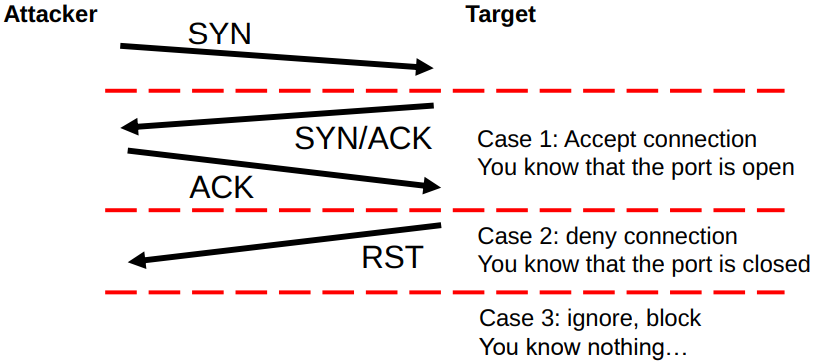
\includegraphics[width=\textwidth,keepaspectratio]{tcp_scan}
	\end{figure}
\end{minipage}
\hfill
\begin{minipage}[t]{0.45\textwidth}
    \subsection{TCP With SYN Only}
    Fast but not supported by the OS (you have to write your own code)
	\begin{figure}[H]
		\centering
		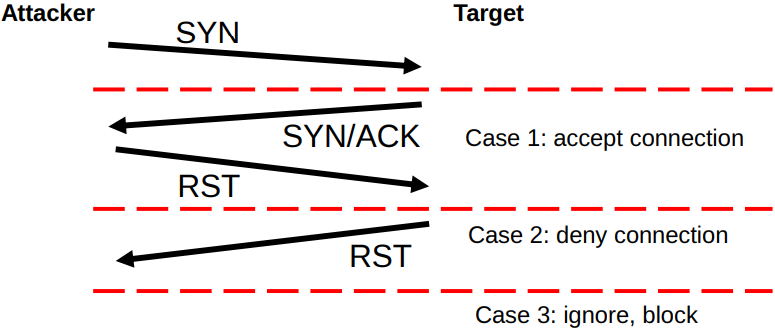
\includegraphics[width=\textwidth,keepaspectratio]{tcp_syn}
	\end{figure}
\end{minipage}

\subsection{TCP XMas-Tree Scan}

\begin{figure}[H]
    \centering
    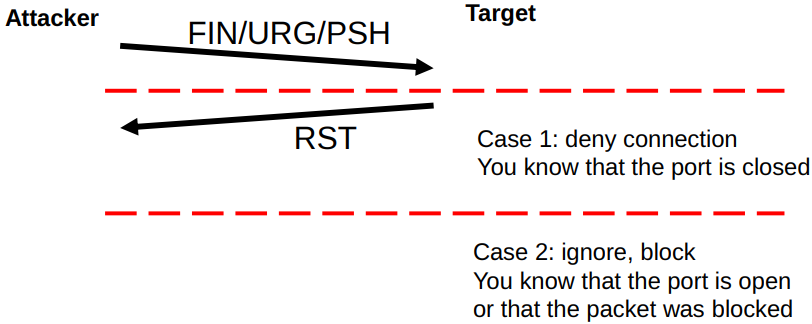
\includegraphics[width=0.5\textwidth,keepaspectratio]{tcp_xmas}
\end{figure}

\section{UDP Port Scan}

UPD is connectionless so the TCP approach does not work. We need to send a packet to the target and :
\begin{itemize}
    \item wait for a negative answer (i.e. '\textit{port unreachable}' ICMP message if UDP port is closed)
    \item wait for a positive answer
\end{itemize}

Easy to implement but not very reliable since UDP packets might be lost or ICMP might be disabled.

\section{Scan Types}

3 main types :
\begin{itemize}
    \item \textblue{Vertical scans} : scan all ports of a target
    \item \textblue{Horizontal scans} : find targets with open ports of interest
    \item \textblue{Block scans} : combination of both
\end{itemize}

\section{Obfuscation}

Scans are also possible for other protocol such as HTTP, smart home automation, ...

Scans might look suspicious for the cybersecurity engineer monitoring the traffic. There are solutions to obfuscate such footprint such as \textit{slow scan, distributed scan, indirect scan, ...}

\subsection{Idle scan}

The goal is to impersonate another computer whose network traffic is very slow or non-existent (hides our address IP as attacker).

It is based on the fact that you can spoof the source IP address in the RCP header of a packer. The target server will therefore respond with a 'SYN/ACK' to the 'zombie' IP which will return a 'RST' containing a 'RST ID' that is sometimes just incremented by 1 each time. We only need to continuously ask the zombie to get a 'RST' in order to see a jump in the IDs

\begin{figure}[H]
    \centering
    \includegraphics[width=0.7\textwidth,keepaspectratio]{idlescan}
\end{figure}

\chapter{Denial Of Service (DoS)}

\textblue{Goal} : overload or crash a server to make the service unavailable to legitimate users.

\section{Types of DoS attacks}

\begin{itemize}
    \item \textblue{Semantic attacks} : make the server non functional by sending requests (e.g. :: sending queries that need a lot of time, that trigger errors, send half a request such that the server will keep the connection open, ... It is cheap for the attacker but requires specific knowledge of the target
    \item \textblue{Brute-force attacks} : overwhelm the server by sending many requests. If coordinated from multiple hosts, we say that it is a Distributed Denial Of Service (DDoS) 
    \begin{figure}[H]
        \centering
        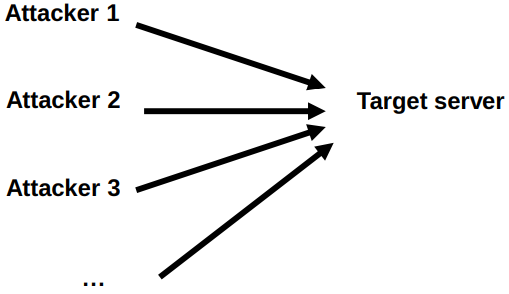
\includegraphics[width=0.3\textwidth,keepaspectratio]{ddos}
    \end{figure}
    \item \textblue{Reflected DoS attacks} : same as DDoS but hides the attacker's IP address with spoofing (DRDoS, uses DNS). Leads to \textit{amplification} : the response is larger that the request (solves the bandwidth problem for the attacker, since DNS queries are very small and answers can be up to 60 times bigger)
    \begin{figure}[H]
        \centering
        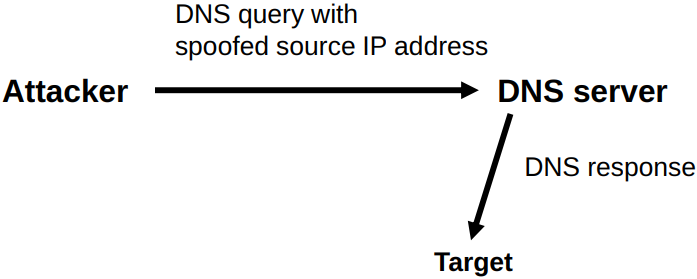
\includegraphics[width=0.4\textwidth,keepaspectratio]{drdos}
    \end{figure}
\end{itemize}

DNS servers are very popular for such attacks because they are open to anybody, they use UDP (perfect for spoofing) and they are made to handle high loads (high computational power).

\section{Mitigation}

\begin{itemize}
    \item Do not let open services that can be misused for DRDoS attacks (switch off unused services, etc. Note that it cannot be done for DRDoS attacks using DNS)
    \item Implement ingress filtering against reflective attacks : router discards packets if source IP does not match network address
\end{itemize}

\section{SYN flooding}

Host $A$ sends many SYN packets to host $B$. It consumes memory in $B$ because the OS allocated data structures for the assumed TCP connections that are not completed. 

$\rightarrow$ Protection with the TCPv4 header \& \textblue{SYN cookies} : $B$ does not allocate memory for the connection before receiving ACK packet from $A$. This ACK packet contains an ACK number, if the cookie is okay and not too old, it is very likely that $A$ sent a SYN before.

\chapter{Domain Name System (DNS)}

DNS is a hierarchical distributed database.

The client queries the \textit{A Resource Record} (IPv4 address) or the \textit{AAA Resource Record} (IPv6 address) of the name to the Local Resolver (only works if the Local Resolver knows the answer).

\begin{figure}[H]
    \centering
    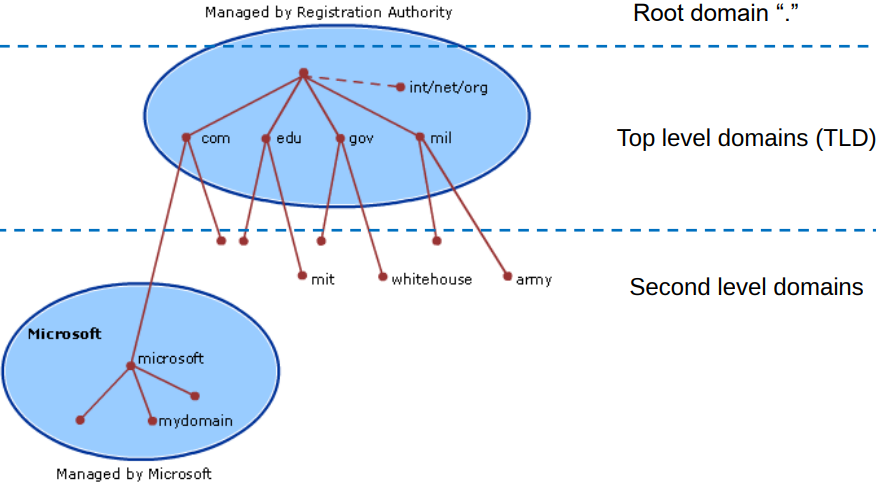
\includegraphics[width=0.49\textwidth,keepaspectratio]{dns_h}\hfill
    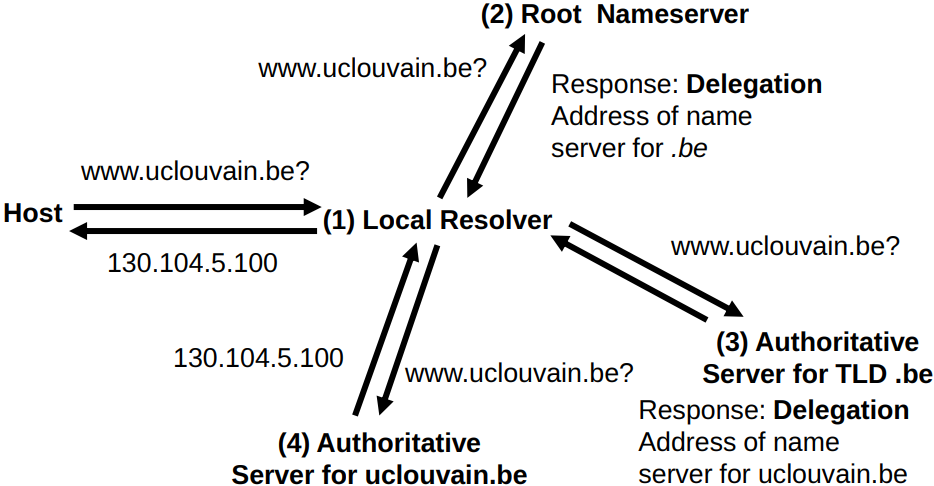
\includegraphics[width=0.49\textwidth,keepaspectratio]{dns_q}
\end{figure}

They are 13 root name servers, that each have a database (\textit{root zone file}), with the IP addresses of the authoritative DNS servers for all Top Level Domains (TDL). These are locally replicated.

To improve performance, the results of recursive DNS queries are caches in local resolvers. DNS records have a Time-To-Live (TTL) defined by the autorotative name server. After that time, they are removed from the cache.

\chapter{Cache Poisoning Attacks}

\section{DNS Cache Poisoning}

\textblue{Goal} : modify the information in the DNS database. The attacker sends a fake response with the spoofed IP address of the authoritative server.

This will direct the victim's traffic to a different host (can present fake website), inspect his activity, etc.).

\subsection{Variant 1}

Attacker asks for a domain name owned by himself. The local resolver adds an additional record in the answer and puts it in the cache of the local resolver.

\begin{figure}[H]
    \centering
    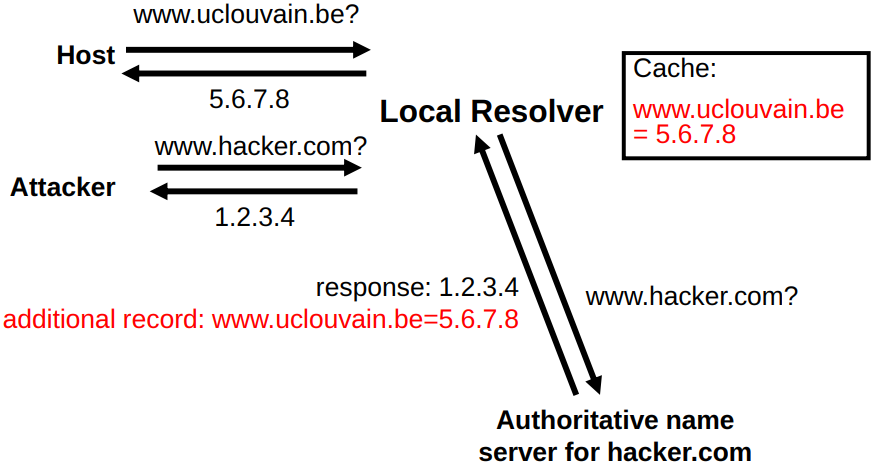
\includegraphics[width=0.49\textwidth,keepaspectratio]{dns_v1}
\end{figure}

Not possible any more thanks to the \textblue{Bailiwick check} : local resolvers accept additional records only if they contain information about the same domain as the request.

\subsection{Variant 2}

Attacker sends his malicious IP address to the local resolver before the answer of the authoritative server (which will be discarded by the local resolver).

\begin{figure}[H]
    \centering
    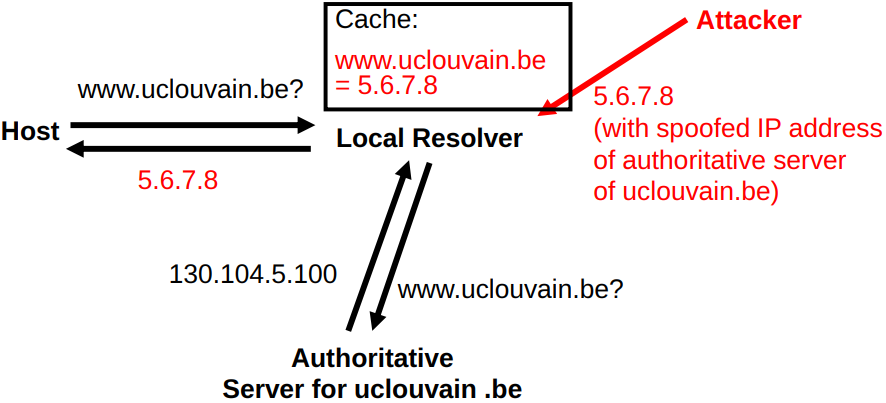
\includegraphics[width=0.49\textwidth,keepaspectratio]{dns_v2}
\end{figure}

Timing is important : the fake answer has to arrive at the local resolver before the real answer. However, the attacker has to guess correctly the port number and the query ID in the fake response (hard)

\subsection{Summary}

Cache poisoning works (or worked) because :
\begin{enumerate}
    \item Resolver accepted additional records without checking
    \item Spoofing is possible since DNS works on UDP
    \item Bad randomization of transaction parameters (query ID and port number)
\end{enumerate}

\section{ARP Cache Poisoning}

Cache poisoning also works for other types of caches where the cache does not verify the identify and authority of the source of the data.

ARP = "DNS for Ethernet addresses".
\begin{enumerate}
    \item Client asks : "Ethernet address of 1.2.3.4 ?"
    \item Anybody who knows the answer can reply : "1.2.3.4 has Ethernet address 01:02:03:04:05:06"
    \item Answers ara cached locally to the client.
    \item[$\rightarrow$] ARP clients also accept unsolicited responses
\end{enumerate}

\chapter{History Stealing and Tracking}

\section{History Stealing}

\textblue{Goal} : website $X$ wants to know what other website users $Y$ has visited before (attack before the privacy of the user).

3 main reasons :
\begin{itemize}
    \item Getting infos about competitors
    \item Preparing a phishing attack
    \item Improve user experience
\end{itemize}

In theory, JavaScript doest allow access to the browser history, the cache content or the cookies stored in the browser (unless they belong to the consulted website). But in reality, a lot of ways exists (some have been fixed years ago, some are still available and some other are "intentional" (i.e : browser extension)).

\subsection{Stealing Through CSS}

Based on the fact that browsers can display visited and unvisited links differently, controlled by user settings and CSS files (ex : red if visited links). An attacker can then just check the color of a link (i.e by checking the display style of an hidden link).

Fixes :
\begin{itemize}
    \item \ctext{lightGray}{getComputedStyle} always returns the unvisited style for links (not enough because of font sizes, ...)
    \item Websites are only allowed to change the color of links (no impact on the layout of the site)
\end{itemize}

\subsection{Timing Attack}

Exploit the fact that some operations take longer than others. Website $X$ executes one of the below operations and measures the time to complete it :
\begin{itemize}
    \item Define a very complex style for visited links, such that they take more time to be displayed
    \item Request an object from website $Y$ (rapidly if in cache) or load website $Y$ into a frame
\end{itemize}

Fixes :
\begin{itemize}
    \item Modern browsers have optimized render engines where display speed difference between styles is very small
    \item Disable the cache / DNS / JavaScript
    \item Cache isolation : ignore the cache if an object is loaded from a different domain name
\end{itemize}

\section{Tracking}

Browsers track users with cookies. Nowadays, websites embed links to tracking services on their web pages (e.g. Google Analytics, ...)

Blocking cookies does not mean that one cannot be tracked : all the information sent in HTTP header fields is enough to identify you.

\textblue{Perma-cookie} : cookie injected into the HTTP requests of users by their Internet Service Provider (ISP) or their mobile phone operator (impossible in HTTPs)

\chapter{Botnets}

Collection of compromised / hijacked machines (bots, zombies) under control of an attacker (botmaster). Machines can be compromised with a malware containing a virus, a worm (a virus that spreads to other computers), ...

Once a machine has been "recruited" for a botnet it is ready to receive instructions from the botmaster (commands, updates, transfer informations, ...). Botmaster operates a \textit{Command-and-Control} server that communicates with the bots.

This is challenging because he has to operate 
\begin{itemize}
    \item without revealing its identify
    \item without raising alarms of admins/users who monitor the traffic of their machines
    \item in a flexible way (ability to find a new C\&C if the first one is shut down)
\end{itemize}

\section{Storm Architecture}

\begin{figure}[H]
    \centering
    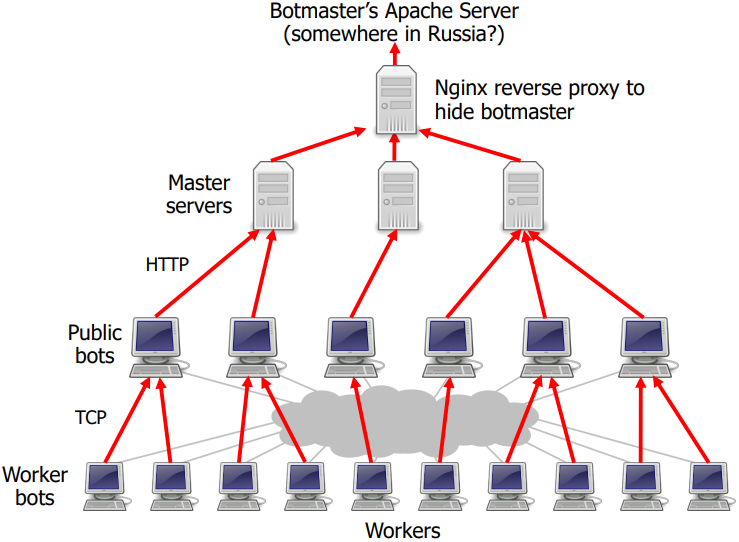
\includegraphics[width=0.5\textwidth,keepaspectratio]{storm_architecture}
\end{figure}

Used for spamming :
\begin{itemize}
    \item \textit{Worker bots} : Computers that request jobs from the master servers and execute them
    \item \textit{Public bots} : Infected computers that are externally accessible
    \item \textit{Master servers} : Compromised computers managed by the botmaster directly and hosted in data centres using an NGINX reversed proxy server to hide the top-level server of the botmaster.
\end{itemize}

To find the master servers, bots resolve a domain name. The IP address of the domain name is rapidly changed, pointing to a compromised computer.

\section{Fight Botnets}

\begin{itemize}
    \item Prevent infection with bot malware (hard)
    \item Take down C\&C servers (hard because of botnet architecture)
    \item Intrude the botnet and send switch-off commands (but modern botnets use encryption and authentication)
    \item Seize the domain names used by the botnet (successful in the past, but not possible today since they generate large lists of possible domains)
\end{itemize}

\chapter{Firewalls}

A firewall tries to improve security by isolating a trusted network from an untrusted network (e.g. isolate intranet from the Internet). It is a checkpoint where all traffic between the two networks has to pass through.

Firewalls can be classified by their :
\begin{itemize}
    \item \textblue{Layer of operation} : Network layer (IPv4, IPv6), Transport layer (UDP, TCP), Application layer (HTTP, ...)
    \item \textblue{Internal state} : stateless or stateful
    \item \textblue{Location} : network or personal (host) firewall
\end{itemize}

\section{Internal State}

\subsection{Stateless Firewall}

These firewalls operate as rule-based packet filters (they look at every packet and decide whether packet should be dropped or forwarded).

Examples :
\begin{itemize}
    \item \ctext{lightGray}{allow tcp 1.2.3.4:1025 $\rightarrow$ 5.6.7.8:80}
    \item \ctext{lightGray}{deny tcp 1.2.3.4:* $\rightarrow$ 5.6.7.8:80}
\end{itemize}

The rules are browsed top-to-bottom and the directions is not taken into account. If no rule matched the traffic the default policy will be applied (default deny/default allow). In general, a default-deny policy is recommended.

A stateless firewall does not know what a TCP connection is. It will therefore drop incoming packets of the outbound TCP connection if configured incorrectly.

\subsection{Stateful Firewall}

A stateful firewall has an internal list "state" of existing connections it has seen previously. If a packet comes in, the firewall checks the list whether the packet belongs to one of the existing connections (basically using a state table like NAT).

It understands the protocol : it knows for example that a SYN packets needs to be followed by a SYNACK and so on. Therefore, they need more resources than stateless firewalls because they have to keep track of the state of connections. State information is removed based on observed packets (FIN-FINACK-...), timeouts or inactive connections.

It is not always trivial to implement a stateful firewall for more complex protocols (like FTP-Active which uses 2 different ports to communicates). Not surprisingly, application-layer firewalls need more resources than lower-layer firewalls (of course, the more complex a firewall, the higher the risk that it has weaknesses or bugs)

\section{Location}

A \textblue{network firewall} is easy to monitor, protects the entire network but does not protect hosts against internal attacks coming from inside the network.

A \textblue{host firewall} requires a large administration overhead if the network contains hundreds of hosts but protects against internal attacks.

It is possible to combine both (expensive network firewall at application layer and fast \& light weight transport layer personal firewall)

\section{DMZ}

Often, a company also need to be reachable from the outside (e.g. web server). With a Demilitarized Zone (DMZ), we accept the fact that hosts exposed to the Internet are less trustable.

\begin{figure}[H]
    \centering
    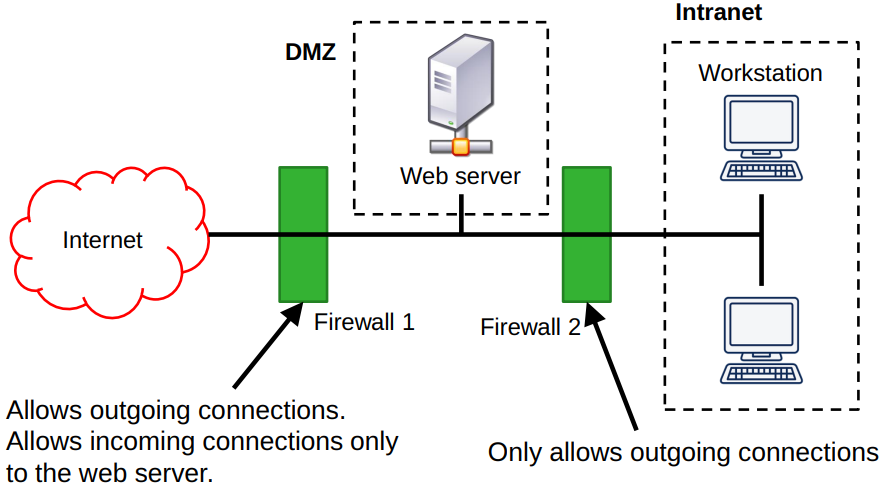
\includegraphics[width=0.5\textwidth,keepaspectratio]{dmz}
\end{figure}

However, DMZ attacks are still possible (e.g. : through connections from the intranet to the web server (database)).

\section{Proxy Firewalls}

Proxies are useful in many situations (as caches, for load balance) as they act as middleman.

Two types of proxies :
\begin{itemize}
    \item \textblue{Transparent proxies} : intercept queries to the original wab server (client is not aware that is not talking to the original)
    \item \textblue{Reverse proxies} : servers that hide the origin servers from the client (client has no knowledge of the original's existence), can handle authentication of clients. Proxies can operate as application firewalls
\end{itemize}

\section{Summary}

\begin{itemize}
    \item \textblue{Deny by default}
    \item \textblue{Principles of least privileges} : only allow what is absolutely needed
    \item \textblue{Choke point} : it is easier to implement security if all data has to go through one point
    \item \textblue{Defence in depth} : deploy multiple defence systems
    \item \textblue{Zoning} : establish trust zones
\end{itemize}

\chapter{Network Address Translation (NAT)}

NAT is how our home network works. You have only 1 public IP address (assigned to your box) and multiple private addresses (assigned to each of the devices in your local network)

NAT's goal is to manipulate packets on network and transport layer to make the translation between one private address and the public address by replacing the source IP address (by the public address) and the source port (by an arbitrary unused port).

Network Address Translation will then keep an internal translation table and do the opposite algorithm for each incoming packet in order to dispatch it to the right device. The complete procedure for outgoing packets is :
\begin{enumerate}
    \item Check if there is a matching entry in the table
    \item If no entre found, insert a new one
    \item Replace address and port number in the packet
\end{enumerate}

You can also add a static table entry (port forwarding) if you for example want to access an internal device from the outside. If there is no matching entry in the table for the incoming packets, it is dropped by default.

\begin{minipage}[t]{0.46\textwidth}
    \section{Advantages}
    \begin{itemize}
        \item Entire network only needs one public IP address
        \item Hosts inside the private network are not any more directly reachable from the internet (not intended as a security solution, every entry in the table "punches a hole" in the perimeter)
        \item NAT is able to hide sequentially incrementing source port number
    \end{itemize}
\end{minipage}
\hfill
\begin{minipage}[t]{0.46\textwidth}
    \section{Drawbacks}
    \begin{itemize}
        \item Violates the separation of protocol layers
        \item Makes network debugging and forensic analysis network traffic harder
        \item An incorrectly implemented NAT might not choose port number randomly and makes them predictable for attacks
        \item Resource intensive
        \item Break the end-to-end principle of Internet (problem for p2p protocols)
    \end{itemize}
\end{minipage}

\section{Attacks}

An attacker \textblue{inside} the company network sends many SYN packets to different IP addresses. This will result of NAT running out of available port numbers, so any new outgoing connection will be blocked.

\chapter{Intrusion Detection Systems (IDS)}

The job of an IDS is to detect intrusion. When an intrusion has been detected, actions can be taken : passive (alarm), or active (block the intruder / counter attack). In larger systems, IDS are often active. However, this can be dangerous if an active IDS takes incorrect decisions (false positives).

\section{Detection Methods}

Two basic principles :
\begin{enumerate}
    \item \textblue{Signature/knowledge/misuse based} : look for patterns/signatures of known attacks. Very precise when the attack is known but hard to detect new attacks.
    \item \textblue{Anomaly/behaviour based} : look for deviations from normal behaviour. Can detect new attacks but it is hard to define "normal behaviour".
\end{enumerate}

\section{Audit source locations}

What kind of data source is the IDS monitoring for suspicious activities ?

\subsection{Host-based IDS}

IDS is located on the host that it should monitor (e.g. anti-virus on a computer)

\begin{minipage}[t]{0.46\textwidth}
    \section{Advantages}
    \begin{itemize}
        \item Very detailed data sources available for every aspect of the monitored system
        \item Encrypted data not a problem if the IDS runs inside the application
    \end{itemize}
\end{minipage}
\hfill
\begin{minipage}[t]{0.46\textwidth}
    \section{Disadvantages}
    \begin{itemize}
        \item Can consume a lot of CPU and memory on the host
        \item Only sees the activity of one single host : the big picture is missing
        \item Cannot stop attacks against the network link of the host (e.g DoS)
    \end{itemize}
\end{minipage}

\section{Network-based IDS}

IDS that monitors the network traffic. It obtains a copy of traffic through the mirror port of a router/switch. It can monitor traffic at different levels of details : connection summaries, packet headers, \textit{Deep Packet Inspection (\textblue{DPI})} (e.g. \textblue{Snort} : compares the monitored traffic against a set of rules and raises an alarm if a rule matches)

\begin{minipage}[t]{0.46\textwidth}
    \section{Advantages}
    \begin{itemize}
        \item Can be deployed on a dedicated machine
        \item Can monitor the activity of the entire network
        \item Flow monitoring scalable to high-speed networks
        \item Flows are good for detection of brute-force DDoS attacks
    \end{itemize}
\end{minipage}
\hfill
\begin{minipage}[t]{0.46\textwidth}
    \section{Disadvantages}
    \begin{itemize}
        \item Only sees the network traffic, not what is happening on the hosts
        \item DPI is expensive and requires special design for high-speed networks
        \item DPI cannot analyse encrypted traffic (e.g. HTTPs)
        \item Flows not very useful for attacks where the packet payload is important
    \end{itemize}
\end{minipage}

Speed of IDS can be improved with more advanced designs :

\begin{itemize}
    \item \textblue{Collaborative IDS} : IDS instances can exchange informations in order to improve detection quality
    \item \textblue{Hierarchical IDS} : small and fast IDS can forward analysis results to bigger IDS for further analysis
\end{itemize}

\chapter{IDS Detection Performance}

An IDS is a binary classifier. It takes some sample and has to decide whether it is normal or malicious. Ideally normal samples are very different from malicious samples.

Ideally, normal samples are very different from malicious samples (left). But in reality, normal and malicious samples can overlap for a chosen metric (right). It is possible to choose another metric, but $0$\% error is in general impossible

\begin{figure}[H]
    \centering
    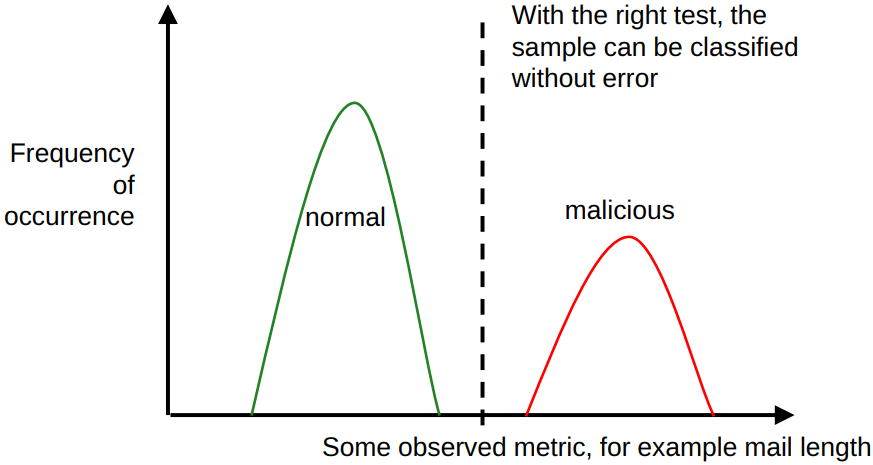
\includegraphics[width=0.48\textwidth,keepaspectratio]{ids_c}\hfill
    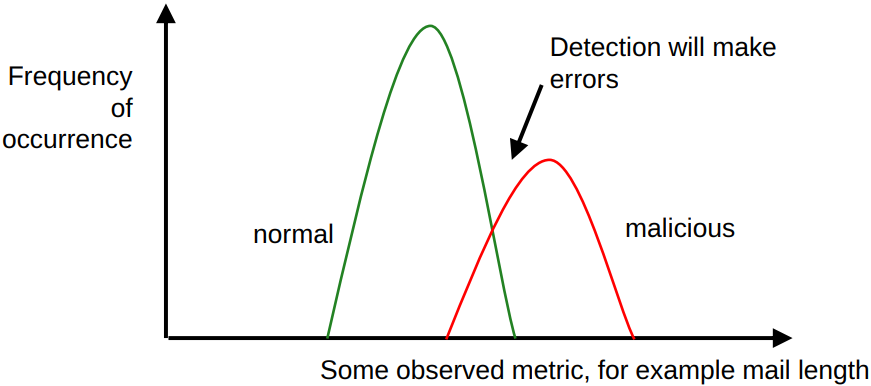
\includegraphics[width=0.5\textwidth,keepaspectratio]{ids_e}
\end{figure}

To know whether an IDS made mistakes, we need a \textblue{ground truth} : an input dataset where each sample is labelled as normal or malicious (very hard to get such datasets, and must contain realistic normal data otherwise the test might become too easy).

The goal is to minimize false positive and false negatives. To do so, we must make a compromise depending on the current security policy.

\section{Confusion matrix}

To test an IDS, we run it on the ground truth dataset and compare the IDS alerts with the labels of the samples. From those results we can produce a confusion matrix.

For example, for a labelled dataset with 20 malicious samples and 80 normal samples:

\begin{figure}[H]
    \centering
    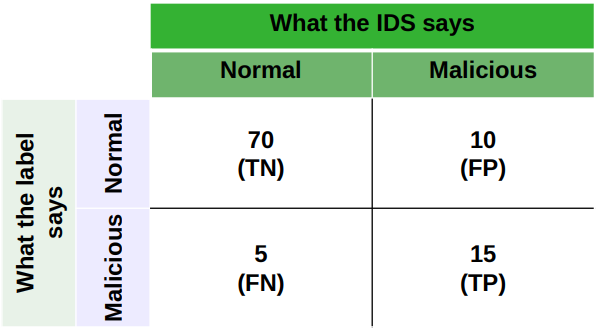
\includegraphics[width=0.5\textwidth,keepaspectratio]{confusion_matrix}
\end{figure}

\section{Tuning}

Ideally, False Positives and False Negatives are very close to 0.
\begin{itemize}
    \item FP : Expensive (alerts have to be checked)
    \item FN : Security risk (unnoticed intrusions)
\end{itemize}

Therefore we need to find a compromise. An acceptable FP and FN rate depends on the security policy.

\section{Receiver operator Characteristics (ROC)}

The dependency of the IDS performance on a specific detection parameter can be visualized by the ROC curve. The goal here is to maximize the space under the curve.

\begin{figure}[H]
    \centering
    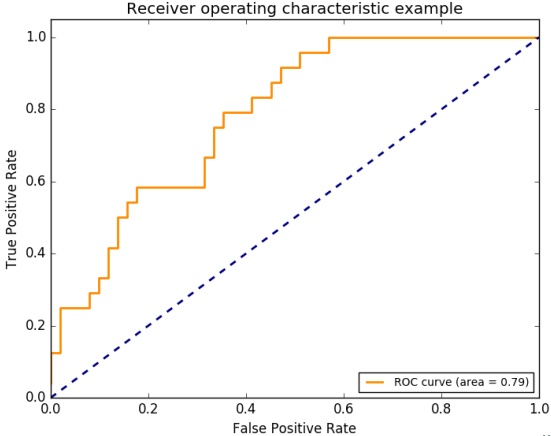
\includegraphics[width=0.5\textwidth,keepaspectratio]{roc}
\end{figure}

\chapter{SPAM and Phishing}

Spam corresponds to unsolicited messages, sent in bulk to many recipients. Typically, the sender address is forged to prevent counter measures.

It is used for multiples reasons:
\begin{itemize}
    \item Advertising products and goods (illegal products, fake products, stolen products, ...)
    \item Fraud schemes (Nigerian prince, "earn money at home", ...)
    \item Recruiting for illegal activities (money mules, re-shippers, ...)
    \item Infection (botnets, ...)
    \item Phishing + spear-phishing
\end{itemize}

Some techniques are used to sell the fake even further, like URL obfuscation (a spoofed website tries to have a genuine looking URL (characters look alike, e.g. I(uppercase i) and l (lowercase L), 0 and O).

How to get e-mail addresses for spamming?
\begin{itemize}
    \item Crawl web pages
    \item Join mailing lists, forums, ...
    \item Hack servers of discussions forums, online communities, ...
    \item Infect a PC and get the entries from their address book
    \item Guess
    \item Buy them (price depends on "quality")
\end{itemize}

It is hard to be successful, since you have to pass the spam filters, convince the user to read the email, to click the link, to stay on the website and buy something or enter sensitive information ($\rightarrow$ very low conversion rate)

How to send spam ?
\begin{itemize}
    \item Use your own SMTP server
    \item Create fake mail accounts at free web mail providers
    \item Use an open mail-relay server (probably blacklisted)
    \item Use infected computers (botnets)
\end{itemize}

\section{Mail Filtering}

Modern filters analyse several aspects of the mail : source IP, URL, mail addresses, keywords, etc. It computes a score for each mail, if the score is above a configurable threshold, the mail is marked as spam.

\subsection{SPF Record}

\textblue{Sender Policy Framework} (SPF), allows the owner of a domain to specify which computers are authorized to send emails with that sender address (can be queried over DNS).

When a SMTP client sends a message to a SMTP server, the client first sends a HELO message with its identify. The server can use SPF to verify whether the sending IP address is authorized or not.

\subsection{Blacklists}

Sender IP address is checked against a blacklist (not sender mail address because it can be spoofed)

Greylisting:
\begin{itemize}
    \item First attempt is rejected
    \item Real mail server will try a second time, spam servers will probably not retry (to save resources)
    \item Several minutes between the two attempts. Gives time for blacklists to register the spam campaign
\end{itemize}

\textblue{SBL} (list of IP of known spammers), \textblue{XBL} (list of IP of hijacked PC). This lists can be downloaded or accessed via DNS.

\ctext{lightGray}{dig +short <ip>.spamhauss.be} : Response specify if IP is blacklisted

Blacklists are filled by spam traps (mail honeypots). This can be hidden emails on web pages.

\subsection{Bayesian filtering}

The principle of this filter is the following :
\begin{enumerate}
    \item Take a large corpus of ($a$) spam mails and ($b$) non-spam mails
    \item Split the mails into tokens (words) and calculate the token frequencies in ($a$) and ($b$)
    \item Based on the result from step 2, calculate for each token the probability that a mail containing the token is spam
    \begin{itemize}
        \item Probability that an e-mail is spam if it contains token $t$ : $P(isSpam | t)$
        \item Bayes theorem :
        \begin{align*}
        P(isSpam | t) &= \frac{P(t | isSpam) * P(isSpam)}{P(t)}\\
                      &= \frac{P(t | isSpam) * P(isSpam)}{P(t | isSpam) * P(isSpam) + P(t | isNotSpam) * P(isNotSpam)}
        \end{align*}
        \item Paul Graham's original mail filter assumed that $P(isSpam) = P(isNotSpam)$ and got the simpler formula :
        \begin{align*}
        P(isSpam | t) &= \frac{P(t | isSpam)}{P(t | isSpam) + P(t | isNotSpam)}
        \end{align*}
    \end{itemize}
    \item For a new mail, look at all its tokens and calculate the probability that the mail is spam
    \begin{itemize}
        \item We consider that a mail $m$ consists of $n$ tokens $t_1, t_2, ..., t_n$
        \item Assuming that tokens appear independently in emails (\textit{Naive Bayer Classifier})
        \begin{align*}
        P(m\ isSpam) &:= \frac{\prod \frac{p_1}{P(isSpam)}}{\prod \frac{p_1}{P(isSpam)} + \prod(1-p_i)P(isNotSpam)}
        \end{align*}
        \item If we assume that $P(isSpam) = P(isNotSpam)$ :
        \begin{align*}
        P(m\ isSpam) &:= \frac{\prod p_1}{\prod p_1 + \prod(1-p_i)}\\
                     &\ \ \ \ \ \text{where }p_i = P(isSpam | t_i)
        \end{align*}
    \end{itemize}
\end{enumerate}

We define $g = 2 * $ token frequency in good mails, and $b = $ token frequencies in bad mails. 

If $g + b \geq $\ctext{lightGray}{$<thresholdEnoughData>$}, then :
\begin{align*}
goodRatio &:= min(1, \frac{g}{totalNumberGoodMails})\\
badRatio &:= min(1, \frac{g}{totalNumberBadMails})\\
result &:= max(0.01, min (0.99, \frac{badRatio}{goodRatio + badRatio}))
\end{align*}

Remarks :
\begin{itemize}
    \item We get a concrete probability instead of an abstract score
    \item Learning the token spam probabilities happens only one in training
    \item There are ways to improve the algorithm (i.e. ignore frequent token such as "the", "on", etc., do not assume independence of tokens (take bigrams), ...)
    \item The factor $2$ for good token is there because is practice we receive more good emails than bad ones
    \item $0.01$ and $0.99$ is to limit the result if a token only appears in good/bad emails
\end{itemize}

\subsubsection{Practical example}

\begin{itemize}
    \item Good 1 : \textit{Thank you for the invitation}
    \item Good 2 : \textit{I send you the offer for our latest product}
    \item Bad 1 : \textit{The latest movies on our servers!}
    \item New : \textbf{Download the latest movies!}
\end{itemize}

\begin{figure}[H]
    \centering
    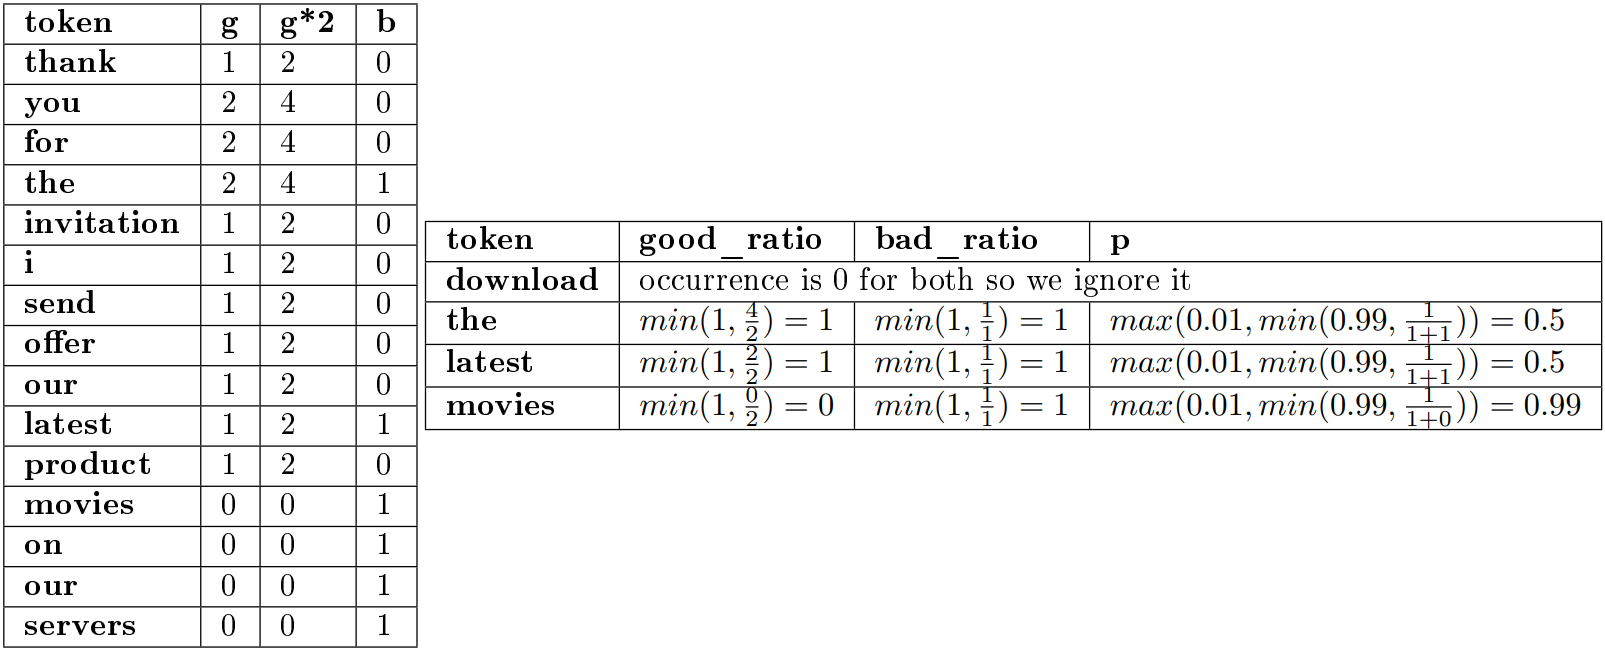
\includegraphics[width=0.9\textwidth,keepaspectratio]{bayes_mail}
\end{figure}

Probability that "new" is spam :
\begin{equation*}
\frac{0.5 * 0.5 * 0.99}{0.5 * 0.5 * 0.99 + (1-0.5) * (1-0.5) * (1-0.99)} = 0.99
\end{equation*}

\chapter{Network Traffic Monitoring}

Network operators keep an eye on the network traffic. IDS also need network traffic to do their job. Detecting attack patterns is difficult, but being able to collect and process network traffic in near real time is already a challenge in itself.

We can measure multiple things :
\begin{itemize}
    \item \textblue{Low level metrics} : can be derived from the packets (packet payload, delay, packet loss, port usage, ...)
    \item \textblue{High level metrics} : harder to get (connectivity between networks, protocol/application usage, availability of services, behaviour, ...)
\end{itemize}

\section{Active measurements}

Generates "probing" traffic, such as network scans, pin packets, HTTP requests to web server to check response time, ... It creates additional load to the traffic but can be done at any scale.

\section{Passive measurements}

Measure by observing existing network traffic (not intrusive, but more challenging). It can be done on a single host via \textit{Tcpdump} or \textit{Wireshark} (promiscuous mode), on switches/routers (create mirror port \& send traffic from mirror port to measurement host), etc.

There might be packet loss, if the output bandwidth cannot handle the amount of traffic of the entire network being monitored. Also, packet capturing is not trivial because in modern networks, the amount of data can be very high (up to 4000GB/hour for high link transports).

\section{Collect And Process Less Informations}

\begin{itemize}
    \item \textblue{Packet header monitoring}
    \begin{itemize}
        \item Still some valuable informations (port numbers, source and destination addresses, TCP flags, packet size, ...)
    \end{itemize}
    \item \textblue{Packet aggregation by flows}
    \begin{itemize}
        \item A flow is a sequence of packets with common properties (source and destination address, port number, layer 3 protocol, ...) that record contains informations about a flow (flow size, flow duration, number of packets, ...)
        \item 2 types of flow monitoring : flow exporter is either part of the router or not. They work as :
        \begin{enumerate}
            \item When packets arrives, calculate hash value for packet's flow key \& lookup in hash table whether the flow exists. Then update/create new flow entry
            \item Entry from the table is remove \& flow record exported (as UDP packet) if :
            \begin{itemize}
                \item Packet observed with special TCP flags (FIN, RST)
                \item Inactivity timeout (no new packets since $x$ seconds)
                \item Activity timeout (entry in table is older than $y$ seconds)
            \end{itemize}
        \end{enumerate}
        \item With flow monitoring, you lose information but you gain space
    \end{itemize}
    \item \textblue{Sampling}
    \begin{itemize}
        \item Do not take every packet
        \item Can be systematic, random, or dynamic
        \item Can also be done in flow-based measurements (before or after doing the flow)
        \item But : sampling can introduce a bias
    \end{itemize}
\end{itemize}

\section{Common Mistakes}

\begin{itemize}
    \item Measuring the wrong thing (e.g. measuring TCP traffic when attacks uses UDP)
    \item Overestimating the capabilities of your measurement system (DDoS can overwhelm the system)
    \item Ignoring measurement bias
\end{itemize}

\begingroup
% Prevent new pages between chapters (in group)
\let\clearpage\relax
\chapter{Honeypots}

\textblue{Goal} : operating fake resources and service to attract attackers to identify/analyse them.

Different types :
\begin{itemize}
    \item \textblue{High interaction honeypots} : imitate the behaviour of real web servers. They are like web servers in an isolated and restricted VM
    \item \textblue{Low interaction honeypots} : just wait for incoming connections
    \item \textblue{Tarpits} : answers very slowly to incoming requests in order to slow down attackers and worms
    \item \textblue{Canary traps} : "secret" information that you intentionally publish to trap attackers
\end{itemize}

Honeypots can be very complex in order to look convincing (they can simulate an entire database/company network honeynet)

\chapter{Network Telescopes}

Researches discovered that even unused IP addresses constantly receive IP packets (from attackers looking for victims, misconfiguration, ...).

Network telescopes run measurements on large unused IP subnetworks and can be used for :
\begin{itemize}
    \item Detecting new attack trends
    \item Indirectly detecting DDoS attacks through their background radiation (backscatter = SYN/ACK packets sent from victim hosts attacked with SYN flooding attacks using spoofed IP addresses)
    \item Identifying typical configuration mistakes
\end{itemize}
\endgroup

\chapter{Symmetric-Key Cryptography}

Cryptography is the art of making a message unreadable. Several algorithm exists.

\textblue{Symmetric ciphers} are efficient (polynomial time) algorithms $E$(ncrypts) and $D$(ecrypt) defined over $K$(ey), $M$(essage) and $C$(iphertext) where :
\begin{align*}
E : K \times M \rightarrow C \text{ and } D : K \times C \rightarrow M\\
\forall m \in M, k \in K : D(k, E(k, m)) = m
\end{align*}
Where $K$, $M$, and $C$ being bit strigs. The key is pre-shared, as both sender and receiver of the message have to know the key $k$.

\section{Perfect Security}

$c$ does not reveal any information about $m$ (besides its length).

For any two messages, $m_1$ and $m_2$, the distributions of $E(k, m_1)$ and $E(k, m_2)$ over all possible keys are identical.

If the symmetric cipher $(E, D)$ is perfectly secure, then key length $\geq$ message length.

\section{One-Time Pad (OTP)}

In OPT, the key $k$ is a random bit string at least as long as the message $m$, and the encrypt and decrypt functions uses XOR :

\begin{equation*}
E(k, m) = k \oplus m \text{ and } D(k, c) = k \oplus c
\end{equation*}

OTP is perfectly secure, but becomes no longer secure if the same key is used twice on two different messages.

\section{Non-Perfect Security}

The requirement that the key has to have at least the same length as the message is not very practical. In practice, one often uses a shorter key $s$ and the key $k$ is generated by a pseudo-random number generator $k = RNG(s)$.

A symmetric cipher used like this is called a \textblue{stream cipher}. It is not perfectly secure (attacker can try all $2^{|s|}$ combination), but infeasible if $|s|$ is long enough (e.g. $\geq 128$ bits).

\section{One-Time Semantic Security}

\begin{itemize}
    \item Let's assume that we have an encryption $E$ and a "Challenge Oracle"
    \item The attacker can send two messages of equal length ($m_1$ and $m_2$) to the Oracle
    \item The Oracle will randomly returns $c = E(k, m_1)$ or $E(k, m_2)$.
    \item Attacker $A$ then tries to guess to which message $c$ belongs
    \item $M_i$ = attacker knows a method that decides that $c$ belongs to message $m_i$
    \item The attacker's advantage over $E$ can be defined over all $k$ as :
    \begin{equation*}
        Adv(A, E) = |Prob(M_1) - Prob(M_2)|
    \end{equation*}
    \item Then, E is semantically secure if $Adv(A, E)$ is negligibly small for all efficient attackers $A$, i.e. no attacker can distinguish $m_1$ and $m_2$ once encrypted in a "reasonable" (polynomial) time
\end{itemize}

\section{Chosen Plaintext Attack}

So far, we assumed that a key is only used once (vulnerable is cipher is deterministic). For multi-use keys, we need stronger security. Same game as in One-time Semantic Security, but attacker can send as many message pairs as they want.

Let's assume the same key is used multiple times :
\begin{enumerate}
    \item We can first send $m_1$ and $m_2$ to the oracle, next time $m_3$ and $m_2$.
    \item If we get the same ciphertext from the oracle, we know that the oracle chose $m_2 \rightarrow$ we have an advantage
\end{enumerate}

Therefore : A cipher with multi-use key cipher can only be secure under CPA if $E$ has some random component.

\section{Cipher Operation Modes}

\textblue{Block ciphers} encrypt the plaintext data by blocks of a certain number of bits $b$. Since block ciphers are deterministic algorithms, this would result in identical ciphertext blocks for identical message blocks.

\textblue{Cipher Block Chaining (CBC)} ) is a mode of block cipher in which the output of the previous block is used to randomize the encryption of the next block. To randomize the algorithm, a publicly shared initialization vector is used (that should be unique for every message)

Many block ciphers are built by applying an invertible transinformation, the "round function", n times to the input. The key is therefore expanded (using another function) to provide different keys for each round.
\begin{figure}[H]
    \centering
    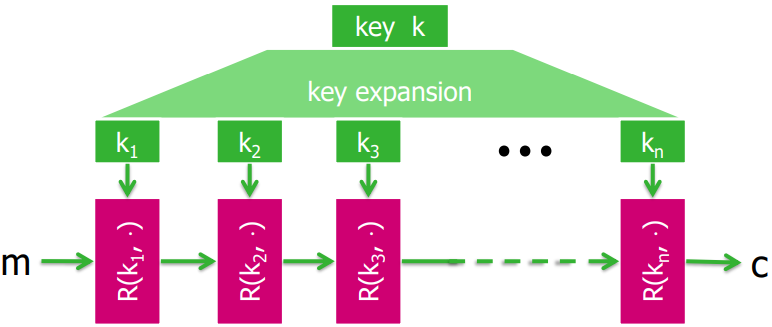
\includegraphics[width=0.3\textwidth,keepaspectratio]{iterated_block}
\end{figure}

\subsection{Data Encryption Standard (DES)}

The original DES has 16 rounds and a 56-bits key. A block of 64 bits is split into two 32-bits blocks $R_0$ (right part) and $L_0$ (left part), then is processed by a \textit{Feistel scheme} :
\begin{align*}
R_i &= f_i(R_{i-1} \oplus L_{i-1})\\
L_i &= R_{i-1}
\end{align*}
\begin{figure}[H]
    \centering
    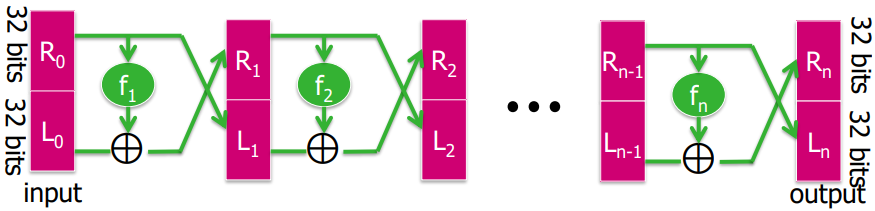
\includegraphics[width=0.5\textwidth,keepaspectratio]{des}
\end{figure}

\subsection{Triple-DES (3DES)}

DES became too short for modern systems. Here, the idea is to run DES 3 times with 3 different keys :
\[
E_{3DES}((k_1, k_2, k_3), m) = E(K_1, D(k_2, E(k_3, m)))
\]
Hence, the size of the key is $3*50 = 128$ bits. This is 3 times slower than DES but much more secure against bruteforce attacks. It is \textit{vulnerable to a "meet-in-the-middle" attack} since the attacker can compute all $2^{56+56}$ possible combination of $D(k_2, E(k_3, m))$ and compare with the remaining $2^{56}$ combination of $D(k_1, c)$

\subsection{Advanced Encryption Standards (AES)}

Established at NIST in 2001. Based on Rijndael cipher and uses CBC with blocks of 128 bits. 3 version (10 rounds, 12 rounds, 14 rounds)

\chapter{Public-Key Cryptography}

\textblue{Idea} : Sender encrypts using a public key $pk$, receiver decrypts using a secret (private) key $sk$.

\begin{figure}[H]
    \centering
    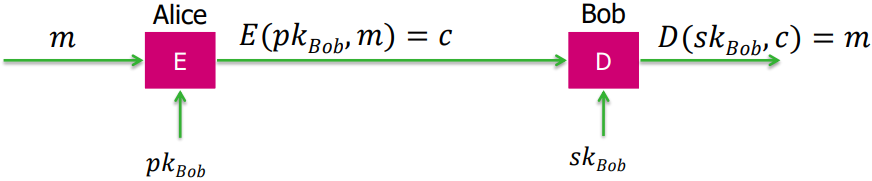
\includegraphics[width=0.6\textwidth,keepaspectratio]{pkc}
\end{figure}

A \textblue{public-key cryptosystem} consists of :
\begin{itemize}
    \item $G$ ! randomized algorithm to generate public and secret keys
    \item $E(pk, m)$ : randomized encryption algorithm
    \item $D(sk, c)$ : deterministic decryption algorithm
\end{itemize}

There is also a consistency requirement : $\forall (pk, sk)$ generated by $G : \forall m \in M : D(sk, E(pk, m)) = m$.

\section{Properties}

\begin{minipage}[t]{0.45\textwidth}
    \textgreen{Pros}
    \begin{itemize}
        \item More formal justification of difficulty available. Hardness is based on complexity-theoretic results of used algorithms
        \item Number of keys : each user only needs one key pair to communicate
    \end{itemize}
\end{minipage}
\hfill
\begin{minipage}[t]{0.45\textwidth}
    \textred{Cons}
    \begin{itemize}
        \item More computationally expensive than symmetric key
        \item More complex system (managing two keys)
    \end{itemize}
\end{minipage}

\section{RSA}

Example for public-key cryptography. Key length should be at least 1024 bits. Is roughly 1000 times slower than DES. In RSA, the key is generated in the following way :
\begin{enumerate}
    \item Choose two randomly large prime numbers $p \neq q$
    \item Calculate the modulus $n := p * q$
    \item Calculate $\varphi(n) = (p-1)(q-1)$
    \item Choose an integer $e$ such that $1 < e < \varphi(n)$ and $GCD(e, \varphi(n)) = 1$ (no common divisor)
    \item Calculate $d$ such that $(d * e)\ mod\ \varphi(n) = 1$
\end{enumerate}

For performance reasons, $e$ is chosen small (not too small, usually it's 65537). We than have the public key $(e, n)$, private key $(d, n)$. $p, q, \varphi(n)$ must also be kept secret (or deleted immediately after key generation).

The encryption and decryption in RSA are :
\begin{itemize}
    \item $E((e, n), m) = m^e\ mod\ n$
    \item $D((d, n), c) = c^d\ mod\ n$
\end{itemize}

\subsection{Security Of RSA}

RSA as presented before is not secure and should not be used in its simple form. Also, it is deterministic, so it can be broken with a chosen plaintext attack. It is also multiplicatively homomorphic ($E(pk, m_1 * m_2 = E(pk, m_1) * E(pk, m_2)$).

To make RSA more secure, long keys are used and short messages are padded with random bits.

In practice, to make RSA more secure,  long keys are used and short messages are padded with random bits. Basically, using a symmetric cipher to encrypt the message and public-key cryptography to encrypt the key of the chosen symmetric cipher.


\section{Diffie-Hellman Key Exchange Protocol}

A secure way to share a secret between two parties $A$ and $B$ :
\begin{enumerate}
    \item $A$ chooses a large prime number $p$ and an integer $1 \leq g \leq p$ and sends $(p, g)$ to $B$
    \item $A$ chooses a secret number $a$, $B$ chooses a secret number $b$
    \item $A$ sends $X = g^a\ mod\ p$ to $B$, and $B$ sends $Y = g^b\ mod\ p$ to $A$
    \item Both sides calculates a shared secret $g^{ab}\ mod\ p$
    \item $A$ and $B$ can now use this shared key for symmetric encryption
\end{enumerate}

Note that is vulnerable to Man in The Middle Attack in step 1. This can be countered with an authentication protocol (e.g. TLS).

\chapter{Cryptographic Hash Functions}

A h\textblue{ash function} takes a variable length input string and return a fixed-length result. Hard function to invert, more expensive to compute than non-crypto hashs (sometimes called "Message Digest"). We want it to have the following properties :
\begin{itemize}
    \item \textblue{One-Way} : given $y$, not feasible to find $m$ such that $H(m) = y$
    \item \textblue{Collision Resistance} : two different messages ($m_1, m_2$) should not have the same hash (i.e. such that $H(m_1) = H(m_2)$)
    \item \textblue{Random Oracle Property} : $H(m)$ is indistinguishable from a random $n$-bit value
\end{itemize}

\section{Collisions}

The birthday paradox says that, given $b$ possibilities and $r$ random samples $x_1, ..., x_r$. What is the probability that there are at least two messages $x_i$ and $x_j$ with $x_i = x_j$ ?

\[
Prob(x_i = x_j) \approx 1 - exp(-\frac{r^2}{2b})
\]

Rule of thumb :

\[
Prob(x_i = x_j) \approx 40\% \text{ when } r = b^{\frac{1}{2}}
\]

Generate $2^{\frac{n}{2}}$ random messages $m_1, ..., m_{2^{\frac{n}{2}}} \in M$. Calculate hashes $t_i = H(m_i)$. According to the birthday paradox, you'll find two messages with the same hash with probability $\approx 40\%$

\textblue{Compression function $f$ (Merkle Damgard)} :
\begin{itemize}
    \item Takes a message block $m[i]$ and result of previous computation $h_{i-1}$ and computes $h_i = f(h_{i-1}|m[i])$
    \item It can be shown that if $f$ is collision-resistant, so is $H$
\end{itemize}

\begin{figure}[H]
    \centering
    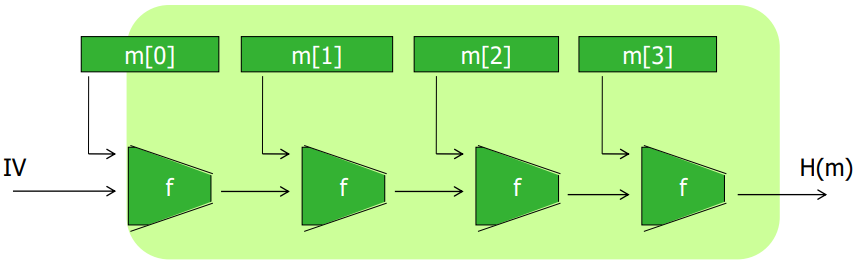
\includegraphics[width=0.6\textwidth,keepaspectratio]{collision}
\end{figure}

\chapter{Message Authentication Code (MAC)}

Basically using a hash function to sign the message + the key.

Given key space $K$, message space $M$ and tag space $T$ :
\begin{itemize}
    \item Signing function calculates tag for a message : $S : \times M \rightarrow T$
    \item Verification function verifies integrity of message : $V : K \times M \times T \rightarrow \{yes, no\}$
    \item Consistency holds : $\forall k \in K, m \in M : V(k, m, S(k, m)) = yes$
\end{itemize}

Procedure :
\begin{enumerate}
    \item Sender calculates tag $t$ for message $m$ with key $k$
    \item Sender sends $(m, t)$ to recipient that computes $r=V(k, m, t)$
    \item If $r \neq yes$ then the message is rejected
\end{enumerate}

Don't append nor prepend the key to the message because it is vulnerable to collisions attack when appending and length-extension attack when prepending.

Solution : Using a PRF to generate a better HMAC.

\chapter{Transport Layer Security (TLS)}

TLS is a protocol to secure data exchange between two hosts (mainly used in HTTPS). Hosts are
authenticated, transfer is encrypted and it supports different crypto protocols.

Basic TLS handshake :

\begin{figure}[H]
    \centering
    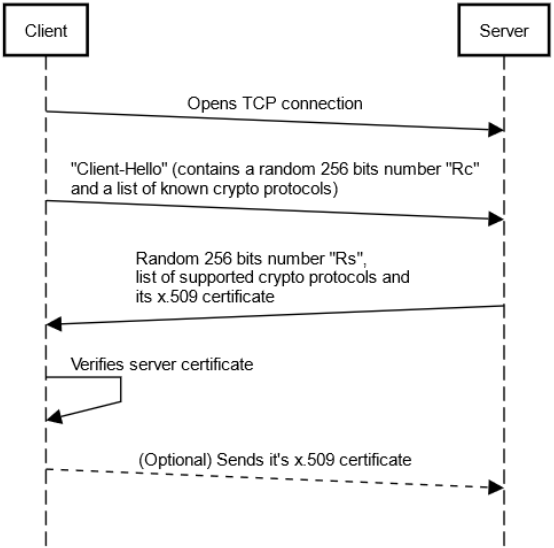
\includegraphics[width=0.5\textwidth,keepaspectratio]{tls_handshake}
\end{figure}

\section{X.509 Certificate}

The X.509 certificate of the server contains its domain name, public key, crypto algorithm for the key, validity period and some other stuff AND which Certificate Authority CA issue the certificate, the signature of this CA and the algo used to generate the signature.

It can be obtained via a Certificate Singing Request :
\begin{enumerate}
    \item Applicant generates a public/private key
    \item Applicant sends a Certificate Signing Request CSR to the CA, with its identity and signed with the applicant's private key
    \item CA verifies identity of application (ID card for example)
    \item CA creates and signs certificate with they own private key
\end{enumerate}

\section{Chain Of Trust}

The certificate is often signed by an intermediate certificate containing the public key of the CA and signed by the higher CA. The most important is that the client knows the public key of the CA and trusts the CA. The root certificate is self-signed. Everyone can self-sign a certificate (useful in an intranet).

To verify a certificate, the client has to :
\begin{enumerate}
    \item Check the identity (must match the server domain name)
    \item Verify all certificates in the chain up to the root \& verify the validity periods
    \item Verify that the certificates have not been revoked
\end{enumerate}

\textblue{SSL/TLS limitations} : it does not protect against DDoS attacks, application vulnerabilities, design error, phishing, compromised CA (attacker getting CA's private key).

\section{TLS 1.3}

TLS up to version 1.2 adds a lot of latency to web traffic : TCP 3-way handshake + TLS handshake = several RTTs (bad for for websites with a lot of objects (pictures, advertisements,...) from different web servers). The negotiation of the ciphers is not signed, meaning that a man in the middle could do a \textit{downgrade attack} (force client and server to use a weak cipher)

In TLS 1.3, improvements were made such as : removing support for some problematic ciphers, negotiation of cipher is now signed, reduce latency of TLS handshake, ...

\subsection{1-RTT mode in TLS 1.3}

\begin{enumerate}
    \item Client $C$ opens TCP connection to server $S$
    \item $C$ sends \ctext{lightGray}{client\_hello}, and makes an assumption about what crypto protocol will be used for the handshake (usually DH)
    \item $S$ computes $K_S$ and replies with the chosen protocol $R_S$, its own part of the data and the certificate encrypted with $K_S$
    \item $C$ verifies certificate of $S$ and computes $K_C$
\end{enumerate}

Data exchange can now be encrypted.

\chapter{Authentication for Client-Server Application}

\section{Session-Oriented Web Applications}

HTTP is a stateless protocol, i.e. the server does not store information about the client. Many applications are session oriented and the application server stores state information for the session.

\subsection{Session Token/Cookie}

The idea is that during login, the server generates a session ID and sends it to
the client as a cookie. The client then the cookie in every request to authenticate (instead of storing it in a cookie, it can be stored in the Local Storage of the browser, but this requires JavaScript.

\begin{minipage}[t]{0.48\textwidth}
    \textgreen{Advantages}
    \begin{itemize}
        \item Session ID can be easily revoked. Just remove it from the server’s internal table
        \item Proven technology
    \end{itemize}
\end{minipage}
\hfill
\begin{minipage}[t]{0.48\textwidth}
    \textred{Disadvantages}
    \begin{itemize}
        \item Session IDs require state to be stored on the server (problematic for applications with many users, each request requires a database lookup on the server etc.)
        \item If stored in the browser as a cookie, the session ID is bound to the domain of the server. Will not work for web applications using multiple domains
    \end{itemize}
\end{minipage}

\subsection{JSON Web Tokens (JWT)}

An extended session ID that contains session information. It is signed by the server, so the attacker cannot modify it. It consists of three parts : header-payload-signature.

\begin{minipage}[t]{0.48\textwidth}
    \textgreen{Advantages}
    \begin{itemize}
        \item Quasi-standardized format that is supported by many libraries
        \item Can be used to build stateless sessions. All state information is put in the payload of the token and sent between client and server
    \end{itemize}
\end{minipage}
\hfill
\begin{minipage}[t]{0.48\textwidth}
    \textred{Disadvantages}
    \begin{itemize}
        \item Because it’s stateless, the only way to make a JWT token invalid is to not accept tokens older than a defined age (using the timestamp in the payload)
    \end{itemize}
\end{minipage}

Therefore, it’s only recommended to use JWT for authentication and to use a session token for the session.

\section{Weakness Of Password Based Client Server Authentication}

The traditional username/password login procedure is too limited for modern applications. 

We introduce \textblue{OAuth2 (RFC 6749)} : an authorization framework for HTTP based services

The resource owner decides what access rights the client will get. The client authorization can be revoked without affecting other clients. The client never sees the resource owner's credentials.

\begin{figure}[H]
    \centering
    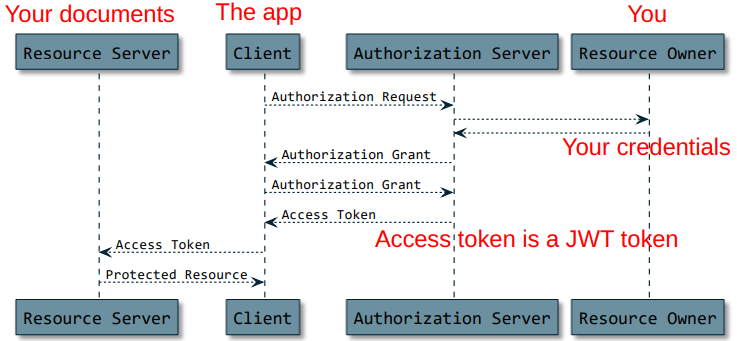
\includegraphics[width=0.55\textwidth,keepaspectratio]{oauth_2}
\end{figure}

\textblue{Token introspection} : resource server sends validation request to authorization server. This could be used by an attacker to find valid tokens (token scanning). To prevent this, the sender of the request also needs a token.

